\chapter{Fundamentação Teórica}\label{cap:fundamentação}

Este capítulo explica de forma breve os conceitos necessários para entender todas as ferramentas usadas no capítulo \ref{cap:metodologia}. 
Para isso, o capítulo é dividido em duas sessões, onde a primeira se baseia em conceitos de processamento de imagem. Já a segunda sessão é dedicada exclusivamente para redes neurais convolucionais e as arquiteturas utilizadas.

\section{Técnicas de Processamento de Imagens}

Este trabalho foi desenvolvido em Python, utilizando a biblioteca \textit{Pillow} para manipular imagens.
As equações que definem as conversões entre espaços são descritas de acordo com a documentação do \textit{Pillow}\cite{clark2015pillow}.
\subsection{Espaço de Cores}
Uma imagem colorida é composta por uma ou mais bandas. 
Usualmente, uma imagem digital em cores é composta por três bandas monocromáticas, onde cada banda armazena uma informação diferente da imagem colorida no pixel p(m,n) da banda. 

Cada banda (ou canal), de largura M pixels e altura N pixels, pode ser considerada como um plano onde um pixel está relacionado a um par de coordenadas inteiras p(m,n) pertencente à banda. 
O valor armazenado na posição m,n no plano indica a intensidade da banda na imagem naquele ponto, usualmente com 256 possíveis valores diferentes de serem armazenados em um byte. 
Onde 0 é a intensidade mais escura e 255 a intensidade mais clara \cite{jaelim, shapiro}.

Existem espaços diferentes de representação de cores, sendo o mais comum o RGB CIE (sigla para \textit{Commission internationale de l'éclairage}) de 1931, 
ou simplesmente RGB (do inglês \textit{Red, Green and Blue}). 
Neste espaço cada cor aparece em seu componente espectral primário correspondente a essas cores, de modo que cada banda armazena unicamente a informação da intensidade do vermelho, verde e azul respectivamente \cite{gonzalez, jaelim}. 
O espaço de cores XYZ-CIE 1931 (XYZ) foi projetado para representar todas as cores visíveis, mesmo as que não são representáveis no RGB. 
As componentes X e Z são elementos sem visibilidade aos olhos humanos, portanto, não existem na práticas como cores \cite{ohta}. 
O componente Y representa a luminância ou a melhor representação monocromática possível da cena originalmente colorida.
% -----------------------

\subsection{Conversões entre RGB e YCbCr}
% https://github.com/python-pillow/Pillow/blob/61a35f94cf8a217db3e67d32db943b05e593e781/src/libImaging/ConvertYCbCr.c#L17-L21

Nestas conversões não há nenhum tipo de alteração nos valores dos pixels no espaço de cor original antes de convertê-los para pixels no espaço de cor desejado.
As equações \ref{eqn:ycrcb_y}, \ref{eqn:ycrcb_cb} e \ref{eqn:ycrcb_cr} mostram a conversão do espaço RGB para YCbCr.
Já as equações \ref{eqn:rgb_r}, \ref{eqn:rgb_g} e \ref{eqn:rgb_b} mostram a conversão do espaço YCbCr para RGB.

\begin{equation}
    \label{eqn:ycrcb_y}
    Y \xleftarrow{} R \cdot 0,29900 + G \cdot 0,58700 + B \cdot 0,11400
\end{equation}
\begin{equation}
    \label{eqn:ycrcb_cb}
    Cb \xleftarrow{} R \cdot -0,16874 + G \cdot -0,33126 + B \cdot 0,50000 + 128
\end{equation}
\begin{equation}
    \label{eqn:ycrcb_cr}
    Cr \xleftarrow{} R \cdot 0,50000 + G \cdot -0,41869 + B \cdot - 0,08131 + 128
\end{equation}

\begin{equation}
    \label{eqn:rgb_r}
    R \xleftarrow{} Y + (Cr - 128) \cdot 1.40200
\end{equation}
\begin{equation}
    \label{eqn:rgb_g}
    G \xleftarrow{} Y + (Cb - 128) \cdot -0,34414 + (Cr - 128) \cdot -0,71414
\end{equation}
\begin{equation}
    \label{eqn:rgb_b}
    B \xleftarrow{} Y + (Cb - 128) \cdot 1,77200
\end{equation}

% \begin{equation}
%     \label{eqn:ycrcb_y}
%     Y \xleftarrow{} 0,299\cdot R + 0,597\cdot G + 0,114\cdot B
% \end{equation}
% \begin{equation}
%     \label{eqn:ycrcb_cb}
%     Cb \xleftarrow{} (B-Y)\cdot 0,564 + delta
% \end{equation}
% \begin{equation}
%     \label{eqn:ycrcb_cr}
%     Cr \xleftarrow{} (R-Y)\cdot 0,713 + delta
% \end{equation}
% onde
% \begin{equation}
%     \label{eqn:ycrcb_delta}
%     delta \xleftarrow{}
%     \begin{cases}
%     128 & \text{para imagens de 8 bits por canal}\\
%     32768 & \text{para imagens de 16 bits por canal}\\
%     0,5 & \text{para imagens normalizadas entre 0 e 1}
%     \end{cases}
% \end{equation}

% -----------------------
\subsection{Transformações de Intensidade no Domínio Espacial}

As transformações de intensidade são funções matemáticas no domínio espacial da imagem, que operam diretamente no valor dos pixels da imagem de entrada \cite{gonzalez}.
Essas funções podem ser representadas pela expressão:
\begin{equation}
    \label{eqn:intensitytransformation}
    g(x,y) = T\left [ f(x,y) \right ]
\end{equation}
onde \textit{f(x,y)} é a imagem de entrada, \textit{g(x,y)} é a imagem de saída e \textit{T} é uma função definida sobre um ponto \textit{x,y} ou sua vizinhança.

Uma das transformações de intensidade mais simples é a transformação linear, onde os valores de intensidade de um canal são multiplicados por uma constante, como representado pela equação:
\begin{equation}
    \label{eqn:linearintensitytransformation}
    i^{'} = \alpha \times i
\end{equation}

Através da equação \ref{eqn:linearintensitytransformation}, a intensidade \textit{i} de um pixel é multiplicada pelo fator de escala $\alpha$, resultando na nova intensidade  $i^{'}$.

% -----------------------
\subsection{Filtragem por Convolução}

Também chamados de máscaras ou kernels, filtros são matrizes de tamanho $m \times n$ aplicadas sobre uma imagem através de multiplicações pelos valores das máscaras e somas, cujos resultados serão os valores da imagem processada.
Suas dimensões e valores que a compõem variam dependendo da característica a ser extraída de cada vizinhança $m \times n$ da imagem, como detecção de bordas ou texturas \cite{shapiro}.
% ----------------------------------------------------------
\section{Redes Neurais Convolucionais}

As redes neurais convolucionais, ou \acrshort{cnn}s, são uma classe especial de redes neurais artificiais que se especializam em processar dados com uma topologia em matrizes \cite{Goodfellow-et-al-2016}. 

Inspiradas pela organização do córtex visual dos mamíferos \cite{hubel1962}, as \acrshort{cnn}s são projetadas para 
%capturar hierarquicamente características espaciais e visuais em imagens, permitindo a extração e o aprendizado de feições cada vez mais abstratas e de alto nível. Nesta seção, abordaremos os fundamentos das CNNs, incluindo suas principais camadas, funcionamento e aplicações em análise de imagens.
extrair características locais que dependem de uma pequena vizinhança na imagem, onde estas pequenas características podem ser usadas por outras camadas para detectar características de maior ordem e extrair informações sobre a imagem \cite{book:Bishop}. 

\acrshort{cnn}s são usadas principalmente para tarefas que trabalham em imagens, como reconhecimento de objetos, segmentação de imagens e detecção de padrões complexos de dados visuais.

O aprendizado de características locais permite que a \acrshort{cnn} reconheça esses padrões em qualquer outro local da imagem,  tornando-a invariante a translação. A utilização de características de uma camada por camadas sucessivas permite que a \acrshort{cnn} aprenda padrões espaciais hierárquicos \cite{book:Chollet}.

% -----------------------
\subsection{Arquitetura de uma Rede Neural Convolucional}

A arquitetura básica de uma \acrshort{cnn} inclui três tipos principais de camadas: convolucional, de pooling e totalmente conectada. 
Uma \acrshort{cnn} típica é formada por pares de camadas de convolução e de pooling empilhadas, que ao final são ligadas a uma camada totalmente conectada.
A Figura \ref{fig:cnn_arch} mostra uma arquitetura genérica de \acrshort{cnn}. 

\begin{figure}[htb]
\centerline{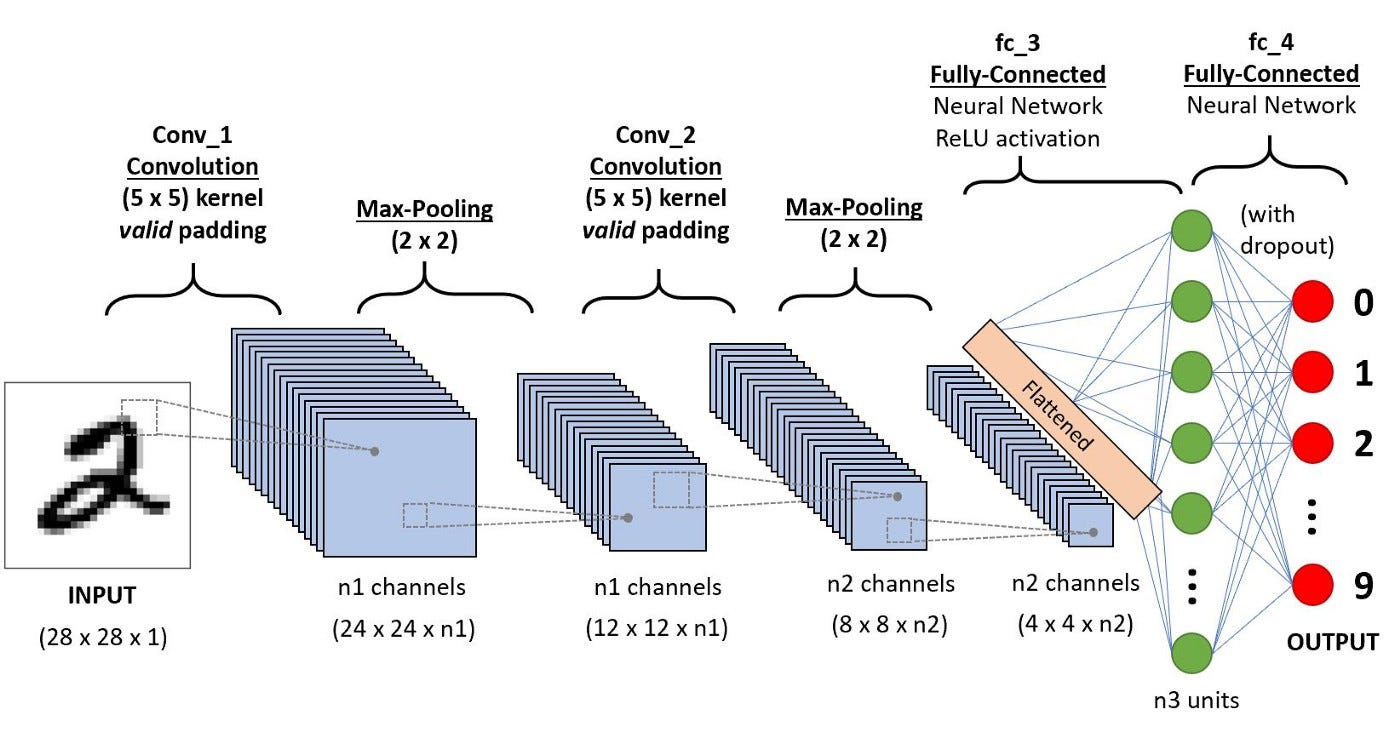
\includegraphics[width=1\linewidth]{images/cnn_placeholder.jpg}}
\caption{Arquitetura de uma \acrshort{cnn} genérica.}
\label{fig:cnn_arch}
\end{figure}

% -----------------------
\subsubsection{Camada Convolucional}

A camada convolucional é o núcleo de uma \acrshort{cnn} e é responsável pela extração de características. 
Para isso pesos na forma de kernels, ou filtros da Análise de Imagem tradicional, 
são aplicados sobre a imagem, onde são escorregados e multiplicados pelos valores dos pixels da imagem de entrada e somados resultando em um pixel para cada kernel, 
usando uma quantidade definida de passos. Esse processo gera os mapas de características, onde cada mapa representa a resposta de um filtro específico a uma região da imagem de entrada. 
Essa camada detecta padrões locais como bordas, texturas ou formas, (de acordo com o kernel usado) que podem ser usados para extrair informações de padrões mais complexos conforme a rede se aprofunda.

A operação de convolução S entre um filtro I e uma entrada K pode ser representada como:

\begin{equation}
    \label{eqn:convolution}
    S(x,y) = \sum_{m}\sum_{n}I(x+m,y+n)K(m,n)
\end{equation}
onde S(x,y) é o mapa de características gerado (saida), I(x,y) representa a entrada local (imagem original) e K(m,n) o kernel aplicado.
% -----------------------
\subsubsection{Camada de Pooling}

%A camada de pooling é utilizada para reduzir a dimensionalidade dos mapas de características, preservando as informações mais relevantes e diminuindo o custo computacional da rede. As operações de pooling ajudam a tornar a rede menos sensível a pequenas variações e deslocamentos na imagem, além de promover uma forma de regularização que reduz o risco de overfitting.

A camada de pooling altera a saída da camada convolucional com um resumo estatístico de uma vizinhança, melhorando a eficiência computacional da rede pela diminuição da dimensionalidade da saída e ajudando a tornar a saída menos variante a translações da entrada.
Este resumo estatístico pode ser feito com diferentes operações. Por exemplo a arquitetura VGG19 \cite{vgg} utiliza \textit{max pooling}, onde a saída é o maior valor na vizinhança analisada. A operação \textit{average pooling} é utilizada no InceptionV3 \cite{inceptionv3}, onde a média da vizinhança é calculada.


% -----------------------
\subsubsection{Camada Totalmente Conectada}

Estas são geralmente as últimas camadas em uma \acrshort{cnn}, sendo responsáveis pela combinação das características extraídas nas camadas anteriores para realizar a classificação final. 
Nesta camada, todos os neurônios estão conectados a cada unidade da camada anterior, como um perceptron multicamadas comum \cite{MURTAGH1991183}. 
O seu aprendizado é feito por um algoritmo de retro-propagação de erro \cite{Rumelhart1986LearningRB}.
% -----------------------
\subsection{Processo de Treinamento de uma CNN}

O treinamento de uma \acrshort{cnn} é realizado por meio de aprendizado supervisionado, onde o modelo ajusta os pesos e vieses das camadas convolucionais (totalmente conectadas) para minimizar a diferença entre as previsões e os rótulos verdadeiros.

A função de perda, que calcula o erro da rede, é derivada e propagada para ajustar os pesos de forma iterativa. 
Este trabalho utilizou a Entropia Cruzada como função de perda, que é definida por:

% Retirado de Goodfellow
\begin{equation}
    \label{eqn:crossentropy}
    H(P,Q) = -E_{P}[log Q]
\end{equation}
onde H(P,Q) é a entropia cruzada da distribuição Q em relação a distribuição P, sendo a distribuição Q o resultado da \acrshort{cnn} e a distribuição P a distribuição de treinamento \cite{mao2023}. 
$E_{P}[.]$ é o valor esperado em relação a distribuição P.

Para minimizar a função de perda, foi usada a descida de gradiente estocástica (\acrshort{sgd}, do inglês \acrlong{sgd}) \cite{ruder2016}. Enquanto a descida de gradiente padrão calcula o gradiente utilizando todo o conjunto de dados, o \acrshort{sgd} utiliza amostras de dados para o cálculo do gradiente na iteração atual.
Dessa forma, a \acrshort{sgd} altera o valor dos parâmetros da seguinte forma:
%Retirado de Bishop
\begin{equation}
    \label{eqn:sgd}
    \omega^{\tau+1} = \omega{\tau} - \eta\Delta{E}
\end{equation}
onde $\omega$ é o peso sendo usado, $\tau$ é o número da iteração, $\eta$ é a taxa de aprendizado e $\Delta{E}$ é o gradiente do erro.

% -----------------------
\subsection{Aprendizado por Transferência}
% IBM, Wikipedia e UFSC referenciam por 'Aprendizado por transferência', AWS e UFRJ referenciam por 'Transferência por aprendizado'
Uma possibilidade importante nas \acrshort{cnn}s é o uso de redes pré-treinadas e aprendizado por transferência (\textit{transfer learning}), 
onde os pesos dos modelos pré-treinados em grandes conjuntos de dados são aproveitados e ajustados para problemas específicos com menos dados, 
reduzindo o tempo de treinamento e melhorando a precisão em aplicações com conjuntos de dados menores. 
Neste trabalho, o aprendizado por transferência baseado no IMAGENET \cite{deng2009imagenet} foi aplicado em todos os modelos avaliados, alterando sua última camada para uma classificação binária.
% -----------------------
\subsection{Visual Geometry Group (VGG)}
A \acrshort{vgg} é uma família de \acrshort{cnn}s que possuem arquiteturas simples. 
Propostas por \cite{vgg}, as \acrshort{vgg}s são compostas por blocos uniformes empilhados com duas camadas convolucionais e uma camada de \textit{pooling}. 
As camadas de \textit{pooling} têm tamanho 2x2 reduzindo a dimensionalidade da convolução pela metade. 

Já as camadas convolucionais compartilham do mesmo tamanho de filtro, sendo estes 3x3. Além disso, cada bloco dobra a quantidade de filtros de suas camadas convolucionais em relação ao bloco anterior. Por exemplo, o primeiro bloco de uma rede \acrshort{vgg} possui 64 filtros 3x3 em suas camada convolucionais, enquanto o segundo bloco possui 128 filtros 3x3.

Este trabalho utilizou a \acrshort{vgg}-19, que indica a existência de 19 camadas de aprendizado, contando não só as camadas convolucionais como as camadas completamente conectadas.
% -----------------------
\subsection{Inception}

Diferente do \acrshort{vgg}, a família \textit{Inception}\cite{inception} de \acrshort{cnn}s utiliza o empilhamento de módulos Inception, onde convoluções de diferentes tamanhos são realizadas no mesmo módulo, especificamente convoluções de 1x1, 3x3 e 5x5. Ao final, tais convoluções são concatenadas junto ao \textit{pooling} da própria entrada, gerando a saída do módulo. 

O \textit{InceptionV3}\cite{inceptionv3} fatoriza convoluções maiores em uma sequência de convoluções menores. A convolução 5x5, por exemplo, é substituída por duas convoluções 3x3, diminuindo a quantidade de parâmetros mas mantendo a expressividade das características extraídas.

Outra modificação implementada no \textit{InceptionV3} foi a utilização do \textit{label smoothing}, onde a confiança do modelo é reduzida para evitar \textit{overfitting}. Isso é feito alterando a probabilidade esperada de cada classe:

\begin{equation}
    \label{eqn:labelsmoothing}
     q(k) = (1-\epsilon )\delta _{k,j}+\frac{\epsilon }{K}
\end{equation}

Onde \textit{j} é a classe correta, \textit{k} é a classe sendo avaliada, $\delta_{k,j}$ é o \textit{Delta de Dirac}, que se torna 1 quando \textit{k = j} e 0 em qualquer outro caso, $\epsilon$ é uma probabilidade de incerteza do modelo, e \textit{K} é o número de classes. Portanto, o \textit{label smoothing} retira da probabilidade \textit{1} da classe correta uma incerteza $\epsilon$ e a distribui igualmente entre as outras \textit{K} classes do problema.
% -----------------------
\subsection{DenseNet}

A característica de maior importância da \textit{DenseNet}\cite{densenet} é que sua arquitetura é baseada em blocos densos, 
que são compostos por camadas convolucionais onde sua entrada recebe a saída de todas as camadas convolucionais anteriores a ela. 
Os blocos densos são ligados por camadas de transição, compostas por uma camada de convolução 1x1 e uma camada de \textit{average pooling} 2x2. 
A arquitetura de uma \textit{DenseNet} simples pode ser vista na Figura \ref{fig:densenet_arch} \cite{densenet}.

\begin{figure}[htb]
\centerline{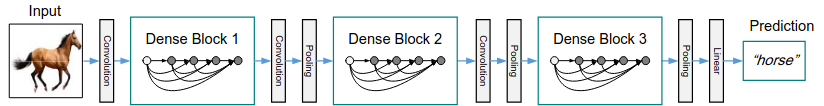
\includegraphics[width=1\linewidth]{images/densenet.png}}
\caption{Arquitetura de uma \textit{DenseNet} genérica\cite{densenet}.}
\label{fig:densenet_arch}
\end{figure}

% -----------------------
\subsection{MobileNet}
A família \textit{MobileNet} de redes neurais foi desenvolvida para utilização por aplicações móveis ou embarcadas \cite{mobilenet}, 
posuindo arquiteturas mais simples e leves em comparação a outras redes neurais profundas, 
mas continuam a oferecer boa performance. Sua maior distinção de outras \acrshort{cnn}s é a introdução de convoluções separáveis em profundidade, que substituem as convoluções tradicionais.

As convoluções separáveis em profundidades fatorizam uma convolução comum em uma convolução em profundidade e uma convolução 1$\times$1, também chamada de convolução pontual. Isso significa que na convolução em profundidade, em vez de aplicar um filtro que abrange todos os canais da janela a qual está realizando a convolução, será aplicada um filtro por canal, onde a saída de cada canal é combinada pela convolução pontual, reduzindo o custo computacional envolvido na convolução.

Além disso, a arquitetura também possui dois hiperparâmetros globais, um multiplicador de largura $\alpha$ e um multiplicador de resolução $\rho$, que servem para reduzir o custo computacional da rede. O hiperparâmetro $\alpha$ serve para afinar a rede neural em cada camada por um fator $\alpha$, aplicado tanto no número de canais de entrada quanto de canais de saída. Já o hiperparâmetreo $\rho$ é aplicado na imagem de entrada e nas representações internas de cada camada, multiplicando-os por $\rho$.

A arquitetura \textit{MobileNetV2}\cite{mobilenetv2} introduz blocos inversos residuais na arquitetura da rede. Este bloco aumenta a dimensionalidade da entrada através de um conjunto de convoluções 1$\times$ 1 e aplica uma convolução em profundidade em seguida, para capturar informações em cada canal expandido. Ao final, uma convolução 1x1 é aplicada para reduzir os canal de volta ao tamanho original.

% -----------------------
\subsection{Visual Transformer (ViT)}
A arquitetura \textit{Visual Transformer}\cite{vit} aplica o conceito de \textit{transformers}\cite{transformer2017} 
utilizados em processamento de linguagem natural para tarefas de classificação de imagens, como alternativa às \acrshort{cnn}s. 
A arquitetura em si é relativamente simples, composta um \textit{transformer enconder}, sem a utilização de um \textit{transformer decoder}, 
que fornece sua saída a um perceptron multicamadas simples (\acrshort{mlp}, do inglês \acrlong{mlp}), sendo este o responsável pela classificação. 
Apesar de simples, nos processos necessários para enviar a imagem para o \textit{transformer} é onde a complexidade da arquitetura aparece.

A Figura \ref{fig:vit_arch} \cite{vit}, mostra a arquitetura de um \acrshort{vit}. 
Diferente de uma \acrshort{cnn} comum, a imagem é dividida em blocos de tamanho fixo denominados \textit{patches}. 
Esses \textit{patches} são transformados em vetores e linearizados. 
Para convertê-los ao espaço de características do modelo, os \textit{patches} passam por um \textit{embedding}, através de uma projeção em um espaço de dimensão fixa. 
Antes de enviar a sequência de \textit{embeddings} ao \textit{transformer}, 
é necessário adicionar um \textit{token} de posicionamento para informar à rede sobre a posição de cada \textit{patch} na imagem original. 
Além desses \textit{token}s, um \textit{token} adicional \textit{class} é colocado no início da sequência, que receberá a saída do processamento realizado pelo \textit{transformer}.

\begin{figure}[htb]
\centerline{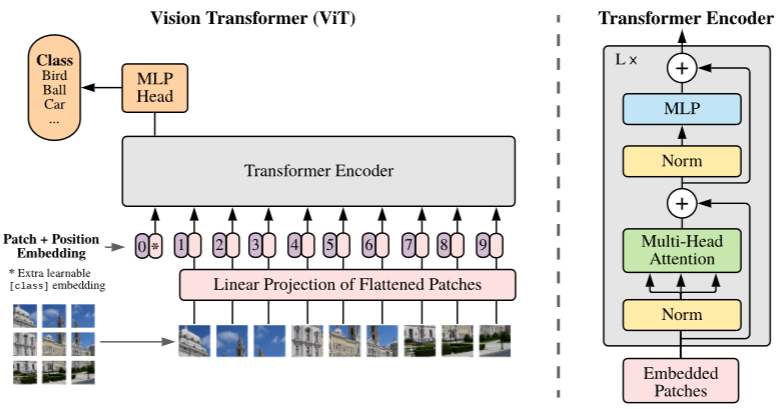
\includegraphics[width=1\linewidth]{images/visual transformer.png}}
\caption{Arquitetura de um \textit{Visual Transformer}\cite{vit}.}
\label{fig:vit_arch}
\end{figure}

O \textit{Transformer} é uma sequência de pares de camadas alternadas, o tamanho dessa sequência de camadas define a profundidade do modelo. 
O primeiro par de camadas consiste em uma camada de normalização, transformando os valores de todos os elementos da sequência para limites predefinidos, e uma camada de \textit{Multi-Headed Self-Attention}, onde é computada uma soma ponderada de entre cada par de elemento do \textit{patch}.
O segundo par de camadas possui uma camada de normalização e uma camada de \acrshort{mlp}, para processar cada elemento do \textit{patch}.

O processamento final do \textit{transformer} é enviado para um \acrshort{mlp} final denominado \textit{MLP Head}, responsável por receber o \textit{token} \textit{class} que representa as informações da imagem aprendidas no \textit{transformer}, e utilizá-lo para gerar a classificação final da imagem.